\section{Laboratory : Integrator Circuits }

Welcome to the time domain !

In this laboratory we study the follower-integrator circuit or FOI.

The FOI is special because its output follows the input at low frequencies, and integrates the input at higher  frequencies. If you did some signal analysis before, the FOI is your low pass filter neuromorphic engineering edition. 

We study the circuit in the time and frequency domain. For large and for small signals. 

\subsection{Time-domain response of small signal}

The experiments starts at steady state. First we need to determine an input voltage that is high enough so that the transamp is capable of operating (i.e. 0.9V). More than that, the input should be corrected by the offset, which is a device specific operation.

At every step in the data collection phase we input this voltage to the circuit minus a small step input (i.e. 0.09V).

In small signals, the output increases exponentially with time based on the following equation :  

$V_{out}(t) = \Delta V_{in}\left(1-e^{-\dfrac{t}{\tau}}\right) + V_{out}(t=0)$.


\begin{figure}[H]
    \centering
    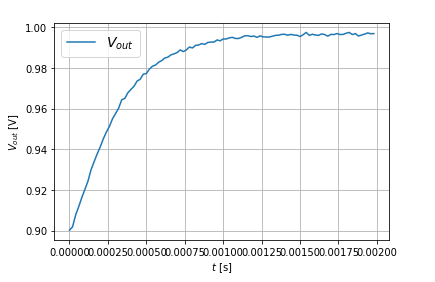
\includegraphics[width=0.95\linewidth]{Figures/ic_smallsignals.png}
    \caption{Step response of the follower-integrator for small signals.}
    \label{fig:basalandcerebellum}
\end{figure}



To extract tau $\tau$, we need to interpolate a function over our data and pass $V_{out}(t)$ to it. 

It should be higher (i.e. 0.0003) than the estimates and the $V_{out}(t=0)$ should be already greater than (i.e. 0.9V). We can recover the moment when the input step takes place by following the curve of $V_{out}$ until it reaches 0V. 

We found a kappa of around 0.8. for this experiment. 

\subsection{Time-domain response of large signal}

The experiment time-domain response over large signals requires a large input step (i.e. 0.3V).

In this regime in the first part of the graph, $V_{out}(t)$ grows linear with time, therefore we can fit a line in this range. 


\begin{figure}[H]
    \centering
    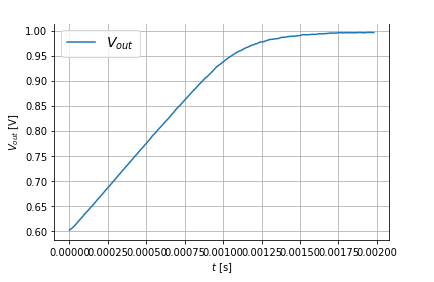
\includegraphics[width=0.95\linewidth]{Figures/ic_largesignals.png}
    \caption{Step response of the follower-integrator for large signals.}
    \label{fig:basalandcerebellum}
\end{figure}



The bias coefficient of the linear fitting gives us the slew rate (i.e 290). The bias current is found by multiplying the slew rate to the capacitance (i.e. 1e-12). We found a bias current 45pA higher than the theoretical expectation.

Tau and kappa in this experiment can be traced back to the linear part of the graph, therefore kappa does not have any significance. 

\subsection{Frequency-domain response}

To measure the curve of the transfer function, we input a sin wave . The output of the FOI, follows the input current. However, it is also possible to change the regime to integrator. The output current of the latter will be translated to the left with respect to the input. 

\begin{figure}[H]
    \centering
    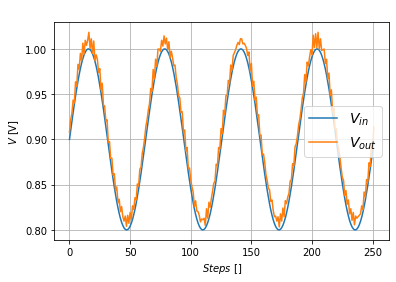
\includegraphics[width=0.95\linewidth]{Figures/ic_freq.png}
    \caption{Follower Integrator, Wave Form}
    \label{fig:basalandcerebellum}
\end{figure}
